\documentclass{article}
\usepackage[utf8]{inputenc}
\usepackage{amsmath, amssymb, amsfonts, amsthm}
\usepackage{mathtools}
\usepackage{mdframed}
\usepackage{cancel}
\usepackage{import, xifthen, pdfpages, transparent}
\usepackage{enumitem}
\usepackage{geometry}
\usepackage{multicol}
\usepackage{hyperref}
\usepackage{mathrsfs}
\usepackage{float}
\usepackage{tikz, pgfplots}
\usepackage{graphicx}
\graphicspath{ {./images/} }
\usetikzlibrary{positioning}
\pgfplotsset{compat=1.18}
\geometry{a4paper, margin=1.5cm}

\newmdenv[
  linecolor=black,
  linewidth=1pt,
  roundcorner=5pt,
  innertopmargin=4pt,
  innerbottommargin=10pt,
  innerleftmargin=10pt,
  innerrightmargin=10pt
]{bxthm}

\theoremstyle{plain}
\newtheorem{thm}{Theorem}[section]
\newtheorem{lem}[thm]{Lemma}
\newtheorem{prop}[thm]{Proposition}
\newtheorem{cor}{Corollary}

\theoremstyle{definition}
\newtheorem{defn}{Definition}[section]
\newtheorem{exmp}{Example}[section]
\newtheorem{xca}[exmp]{Exercise}

\theoremstyle{remark}
\newtheorem{rem}{Remark}
\newtheorem{note}{Note}
\newtheorem{case}{Case}

\newcommand{\incfig}[2][\columnwidth]{%
    \def\svgwidth{#1}
    \import{./figures/}{#2.pdf_tex}
}

\begin{document}
\begin{titlepage}
    \centering
	{\textsc{Università degli Studi della Basilicata} \par}
	\vspace{2cm}
    {\huge\bfseries Tracce dell'esame di Geometria\par}
    \vfill
	{\Large\itshape Donato Martinelli\par}
	{\large \today\par}
\end{titlepage}

\tableofcontents

\newpage

\section{26-11-2019}

\begin{enumerate}
\item
Risolvere il seguente sistema di equazioni lineari al variare del parametro $\lambda \in \mathbb{R}$:
\[
\begin{cases}
(\lambda + 1)X_1 + X_2 + X_3 - X_4 = 0 \\
(2 - \lambda)X_1 + (2 + \lambda)X_2 + 2X_3 - (\lambda + 1)X_4 = \lambda \\
-X_1 - X_2 - (\lambda + 1)^2 X_3 + X_4 = 1 - \lambda
\end{cases}
\]

\item
Si consideri l'operatore lineare 
\[
F : \mathbb{R}^3 \rightarrow \mathbb{R}^3 ,\quad \begin{pmatrix}x\\y\\z\end{pmatrix} \mapsto \begin{pmatrix}x - y + 2z\\2x - z\\3x - y + z\end{pmatrix}
\]
\begin{enumerate}
    \item[i)] Verificare se $F$ è diagonalizzabile.
    \item[ii)] Determinare una base di $\mathrm{Im}(F)$. Determinare una base di $\ker(F)$.
    \item[iii)] Verificare se risulta $\mathbb{R}^3 = \mathrm{Im}(F) \oplus \ker(F)$.
    \item[iv)] Dato $\mathbf{W}=\langle(1,2,3)\rangle$, determinare una base del sottospazio vettoriale $F^{-1}(\mathbf{W})$.
\end{enumerate}

\item
Rispetto alla base canonica sia data la forma quadratica
\[
q : \mathbb{R}^2 \rightarrow \mathbb{R},\quad (x, y) \mapsto x^2 + 2hxy + y^2\quad h\in\mathbb{R}.
\]
\begin{enumerate}
    \item[i)] Dire per quali valori di $h$ tale forma è definita positiva.
    \item[ii)] Posto $h = 3$, determinare una forma canonica per $q$, precisando la base rispetto a cui essa si realizza.
\end{enumerate}

\item
Nello spazio euclideo $\mathbb{E}^3$ dotato di un fissato riferimento cartesiano ortogonale monometrico, sia $r$ la retta congiungente i punti $A = (1, -1, 1)$, $B = (2, 0, 1)$ e sia $\pi$ il piano di equazione cartesiana $2X - T + Z + 1 = 0$.

\begin{enumerate}
    \item[i)] Determinare la proiezione ortogonale $r'$ di $r$ su $\pi$.
    \item[ii)] Determinare il piano $\tau$ contenente $r'$ ed il punto $R = (0, 0, 1)$.
    \item[iii)] Determinare la retta $t$ passante per $R$, contenuta in $\tau$ e ortogonale a $r'$.
    \item[iv)] Determinare il piano contenente la retta $t$ e parallelo alla retta $r$.
\end{enumerate}
\end{enumerate}

\vspace{10pt}

\paragraph{Soluzione}
\begin{enumerate}
    \item 
    Scriviamo la matrice orlata associata al sistema. 
    \[\begin{pmatrix}
        (\lambda+1)&1&1&-1&0\\
        (2-\lambda)&(2+\lambda)&2&-(\lambda+1)&\lambda\\
        -1&-1&-(\lambda+1)^2&1&(1-\lambda)
    \end{pmatrix}\]
    Determiniamo gli insiemi di appartenenza delle matrici.
    \[A=\begin{pmatrix}
        (\lambda+1)&1&1&-1\\
        (2-\lambda)&(2+\lambda)&2&-(\lambda+1)\\
        -1&-1&-(\lambda+1)^2&1
    \end{pmatrix}\in M_{3,4}(\mathbb{R}),\]\\
    \[B=\begin{pmatrix}
        (\lambda+1)&1&1&-1&0\\
        (2-\lambda)&(2+\lambda)&2&-(\lambda+1)&\lambda\\
        -1&-1&-(\lambda+1)^2&1&(1-\lambda)
    \end{pmatrix}\in M_{3,5}(\mathbb{R}).
    \]
    Per verificare se il sistema è compatibile, utilizziamo il teorema di K.R.C.
    Notiamo che $1\leq r(A),r(B)\leq 3 $. 
    Procediamo con il metodo dei minori orlati. 
    Sia $M=B(1\,3\,|1\,2)$, $\det(M)=-\lambda\neq0 \iff \lambda\neq0$.
    perciò $2\leq r(A),r(B)\leq 3 $. 
    Procediamo con l'orlare $M$, 
    \[M_1=B(1\,2\,3\,|\,1\,2\,4), M_2=B(1\,2\,3\,|\,1\,2\,5),\quad M_1\in A,B,\;M_2\in B,\,M_2\notin A.\]
    calcoliamo i determinanti poichè $M_1,M_2\in A$, ed essendo il determinante $\det(M_1)=\lambda\neq0\iff \lambda\neq0$, 
    abbiamo che $r(A)=r(B)=3$. Perciò per KRC il sistema è compatibile e ammette $\infty^{4-3}=\infty^1$ soluzioni.
    Risolviamo con cramer.
    \begin{center}
    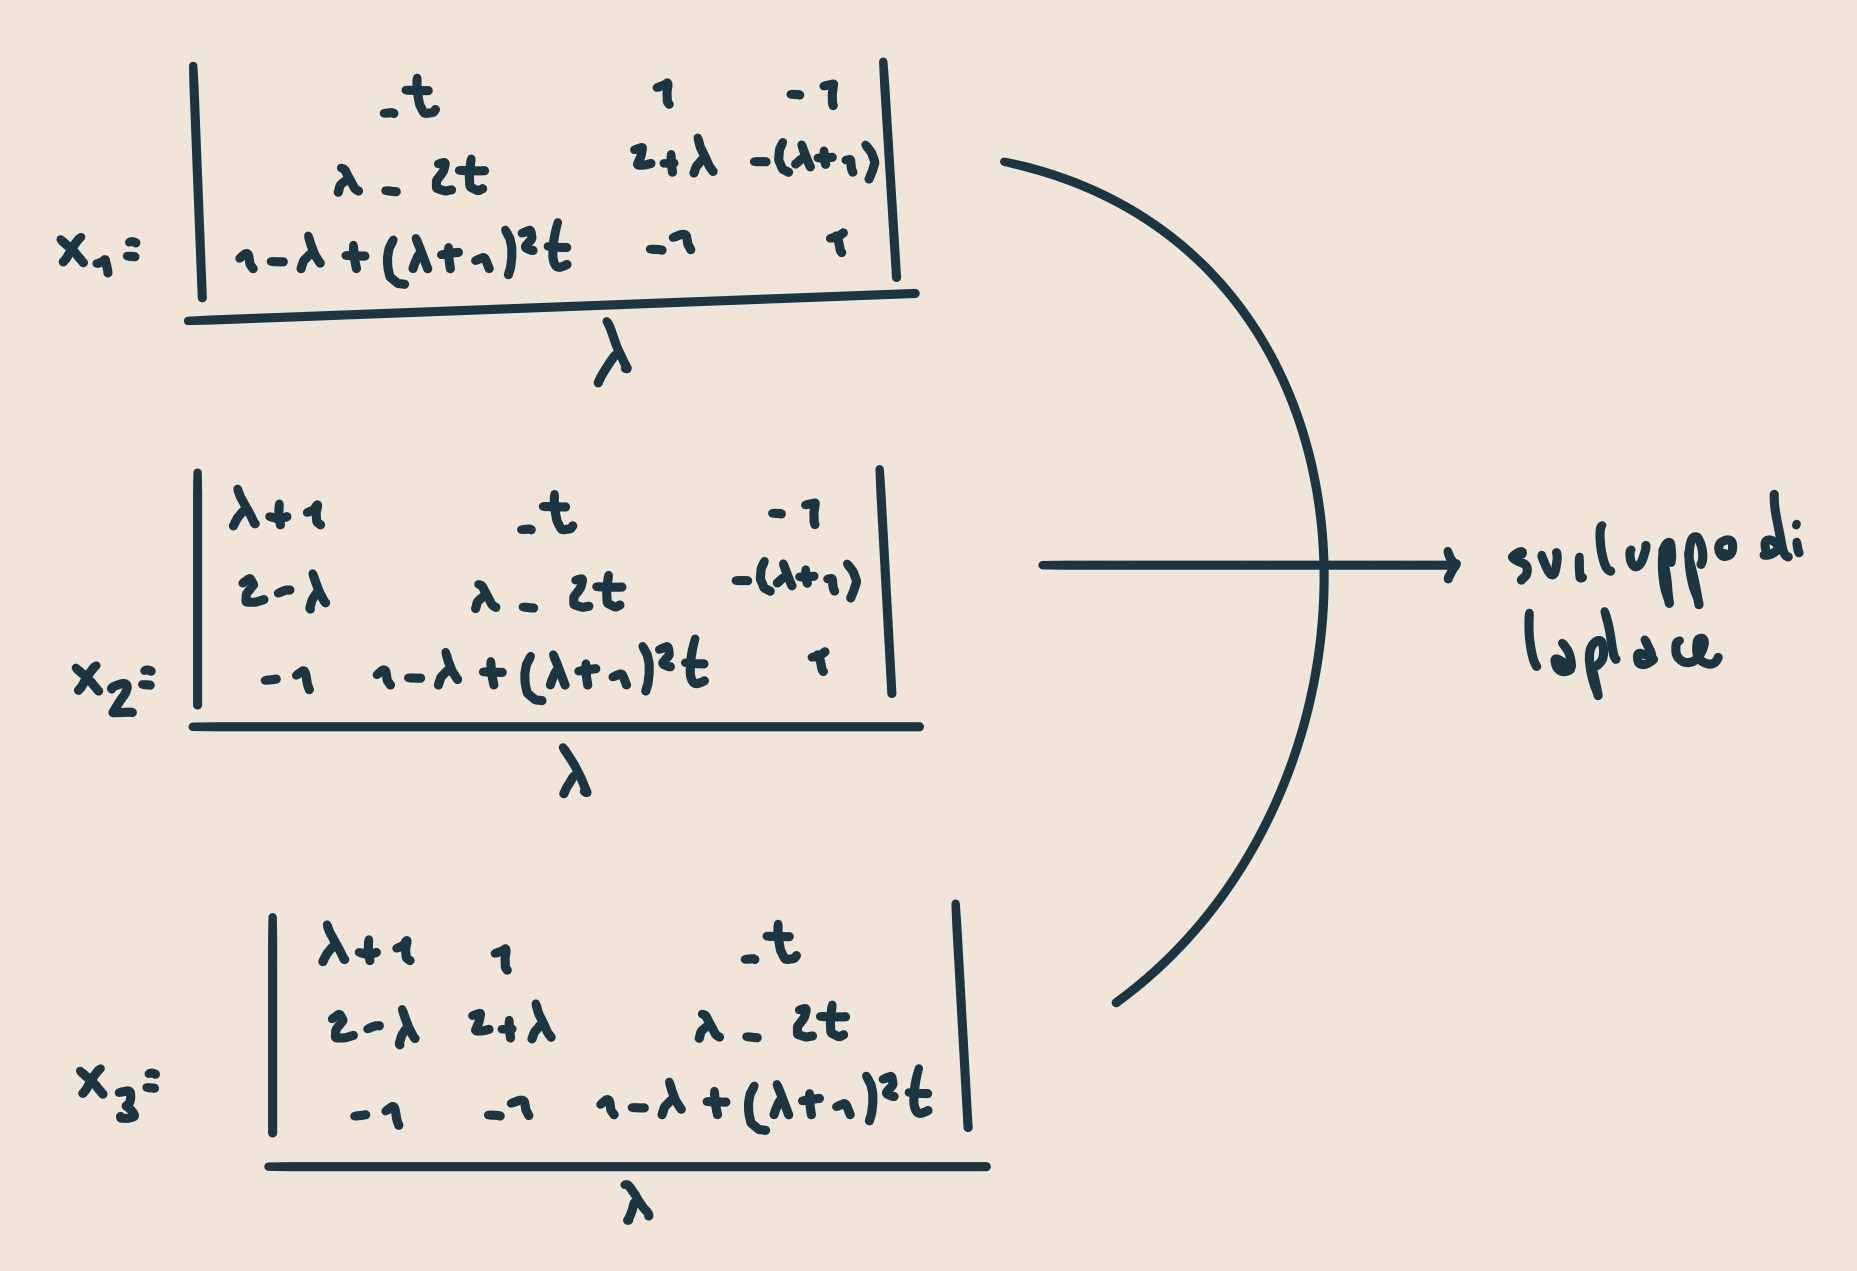
\includegraphics[scale=0.2]{crameruno.jpg}    
    \end{center}
    Calcoliamo i determinanti con Laplace, e otterremo:
    \[(x_1,x_2,x_3,x_4)=\left(\dfrac{\lambda^2t+2\lambda t+1-\lambda}{\lambda},\dfrac{\lambda^4t+5\lambda^3+6\lambda^2t-3\lambda t+\lambda^3-\lambda^2t+4\lambda-1}{\lambda},t,\lambda^3t+6\lambda^2t+9\lambda t-2\lambda+4\right)\;\lambda\in\mathbb{R}.\]
    Se $\lambda=0$, avremo
    \[\begin{pmatrix}
        1&1&1&-1&0\\
        2&2&2&-1&0\\
        -1&-1&-1&1&1
    \end{pmatrix},\]
    Moltiplicando la terza riga per -1, otteniamo il che primo membro di entrambie è uguale, ma non possiamo dire lo stesso per il secondo, dunque il sistema è incompatibile.
    \item 
    \begin{enumerate}
        \item[i)] Scriviamo la matrice associata ad F rispetto alla base canonica 
        \begin{align*}
            \begin{pmatrix}1\\0\\0\end{pmatrix} &\mapsto \begin{pmatrix} 1\\2\\3 \end{pmatrix}\\
            \begin{pmatrix}0\\1\\0\end{pmatrix} &\mapsto \begin{pmatrix} -1\\0\\-1 \end{pmatrix}\\
            \begin{pmatrix}0\\0\\1\end{pmatrix} &\mapsto \begin{pmatrix} 2\\-1\\1 \end{pmatrix}
        \end{align*}
        Otteniamo dunque 
        \[M_{EE}(F)=\begin{pmatrix}
        1&-1&2\\
        2&0&-1\\
        3&-1&1
        \end{pmatrix}=A\]
        Calcoliamo gli autovali, ossia le radici del polinomio caratteristico
        \[|A-\lambda\mathbf{I}_3|=\begin{vmatrix}
        1-\lambda&-1&2\\
        2&-\lambda&-1\\
        3&-1&1-\lambda
        \end{vmatrix}=\cdots=-\lambda(\lambda^2-2\lambda-4).\]
        Lo spettro di $F$ è $\{0,1-\sqrt{5},1+\sqrt{5}\}$. Poichè $F$ ha $3$ autovalori distinti, allora l'endomorfismo è diagonalizzabile.
        \item[ii)] 
        Una base e la dimensione di $\ker(F)$ coincidono con una base e una dimensione dello spazio delle soluzioni del sistema omogeneo 
        $A\mathbf{x}=\mathbf{0}$. Applicando Gauss-Jordan arriviamo al fatto che il sistema possiede $\infty^1$ soluzioni date da $(x_1,x_2,x_3)=t(1,5,2)$.
        otteniamo dunque che $\ker(F)=\langle\begin{pmatrix}1,5,2\end{pmatrix}\rangle$ e dunque $\mathrm{B}_{\ker(F)}=\{\begin{pmatrix}1,5,2\end{pmatrix}\}$.
        e la sua dimensione è $1$ per la cardinalità della base o anche da $\infty^{\textcolor{red}{1}}$.
        Poichè $\dim(\ker(F))$, per il teorema 4.15 avremo che $r(F)=3-\ker(F)=3-1=2$. $r(F)$ è anche uguale ad $r(A)$. Una sua base sarà costituita da due colonne di $A$
        \[\mathrm{B}_{\mathrm{Im}(F)}=\{\begin{pmatrix}1\\2\\3\end{pmatrix},\begin{pmatrix}-1\\0\\-1\end{pmatrix}\}.\]

        \item[iii)] 
        Due sottospazi sono supplementari se e solo se sono in somma diretta. In questo caso se 
        \[\mathrm{Im}(F) + \ker(F)=\mathbb{R}^3 \quad\land\quad \mathrm{Im}(F) \cap \ker(F)=\emptyset.\]
        Dunque uniamo le basi, verifichiamo che queste siano un sistema di generatori prendendo il sistema 
        \[ \begin{cases}a-b+2c=x\\5a-c=y\\2a+b+c=z\end{cases} \]
        La matrice dei coefficienti è 
        \[\begin{pmatrix}
        1&-1&2\\
        5&0&-1\\
        2&1&1
        \end{pmatrix}.\]
        Poichè $1\leq r(A),r(B)\leq 3$, deduciamo che se $\det(A)\neq0$, allora $r(A)=r(B)$, e quindi per KRC il sistema è compatibile, ciò significa che per ogni vettore in $\mathbb{R}^3$, esiste una terna tale per cui il vettore è uguale alla combinazione lineare della base. 
        Oltre a ciò bisogna verificare che i tre vettori siano linearmente indipendenti, e dunque dobbiamo risolvere 
        \[ \begin{cases}a-b+2c=0\\5a-c=0\\2a+b+c=0\end{cases}\implies\begin{cases}a-b+2c=0\\c=5a\\b=-7a\end{cases}\implies \begin{cases}a=0\\b=0\\c=0\end{cases},\]
        dunque lo sono e quindi l'insieme di vettori $\mathrm{B}_{\mathrm{Im}(F)}\cup\mathrm{B}_{\ker(F)}$ è una base di $\ker(F)+\mathrm{Im}(F)$, la sua dimensione è $3$ che è uguale a $\dim(\mathbb{R}^3)$, segue dunque che 
        $\mathrm{Im}(F)+\ker(F)=\mathbb{R}^3$. Per la formua di Grassmann si ha 
        \[\dim(\mathrm{Im}(F)\cap\ker(F))=\dim(\mathrm{Im}(F))+\dim(\ker(F))-\dim(\mathrm{Im}(F)+\ker(F))=2+1-3=0,\]
        e dunque $\mathrm{Im}(F) \oplus \ker(F) = \mathbb{R}^3$.

        \item[iv)] Questo non tanto l'ho capito ma suppongo io debba fare più esercizi.
        
        
    \end{enumerate}
\end{enumerate}



\end{document}
